 \section{Durchführung}
\label{sec:Durchführung}

\subsection{Aufbau}

Der Versuchsaufbau ist in Abbildung \ref{fig:aufbau} dargestellt.
Ein He-Ne-Laser mit einer Wellenlänge von
\begin{align}
  \lambda = \SI{633}{\nano\meter}
\end{align}
trifft auf einen Einzel- oder Doppelparallelspalt und wird dort
gebeugt. In
\begin{align}
L = \SI{1}{\meter}
\end{align}
vom Spalt entfernt ist ein
lichtempfindlicher Detektor positioniert, der mit einem Verschiebereiter
in Spaltbreite-Richtung verschoben werden kann.
Mit einem Amperemeter kann für jede Detektorposition die Stromstärke
abgelesen werden.

\begin{figure}
  \centering
  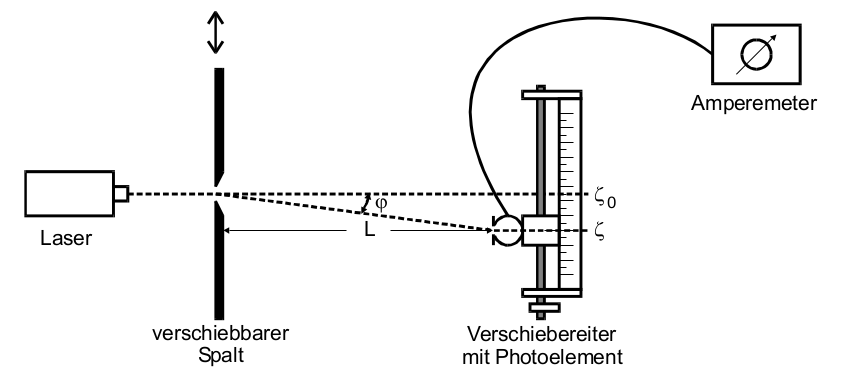
\includegraphics[height=5cm]{MeinePics/Aufbau.png}
  \caption{Versuchsaufbau.\cite{anleitung}}
  \label{fig:aufbau}
\end{figure}

\subsection{Messprogramm}

\subsubsection{Messungen mit dem Mikrometer}

\begin{enumerate}

\item Zunächst wird das auf dem Mikrometer angezeigte Kästchen mit Hilfe
des Objektmikrometers auf dem Objekttisch auf einen Millimeter geeicht und
die Vergrößerung notiert.

\item Die Spaltbreite kann gemessen werden, indem das auf dem Mikrometer
angezeigte Kästchen durch Vergrößerung genau auf die Spaltbreite angepasst
wird.

\item Für insgesamt drei verschiedene Einzelspalte und einen Doppelspalt
wird die Vergrößerung gemessen und notiert.
Mit einem Dreisatz kann daraus die Spaltbreite bestimmt werden.

\end{enumerate}

\subsubsection{Dunkelstrommessung}

Da die Photodiode einen Offset hat, muss eine Dunkelstrommessung bei
ausgeschaltetem Laser durch geführt werden. Der Wert wird dann von allen
Stromstärke-Messwerten abgezogen.

\subsubsection{Spaltmessungen}

\begin{enumerate}

\item Zunächst wird die Detektorstellung $\xi_0$, an der der ungebeugte Strahl
auftrifft, bestimmt.

\item Für drei verschiedene Einzelspalte werden jeweils 51 Messwerte für
Stromstärke und Position bei eingeschaltetem Laser aufgenommen.

\item Für einen Doppelspalt werden insgesamt 81 Messwerte für Stromstärke
und Position aufgenommen.

\item Mit
\begin{align}
  \varphi \approx \tan{\varphi} = \frac{\xi - \xi_0}{L}
\end{align}
können aus den Positionen die Winkel bestimmt werden.

\end{enumerate}
